%! Author = Saeid Yazdani
%! Date = 3/27/2024


\section{Diagnosis of \acs{ATE} \acs{DPS} Units}
\label{sec:diagnostic-problems-ate-dps}

The analysis of the \ac{DUT} socket unveils if all specified values are met
and due to the presence of multiple ground and supply pins in parallel,
wiring influences between support capacitors (both discrete and power planes)
and the \ac{DUT} socket are minimal.

\begin{itemize}[topsep=8pt,itemsep=4pt,partopsep=4pt, parsep=4pt]
    \item \ac{DPS} power supplies may produce large error voltages in the
    leading and trailing sections of the supply waveform.
    The size and number of error spikes will depend on the program code.
    Only using sophisticated \ac{VDUT} measurements we can predict the behavior
    under real test conditions.

    \item Many \ac{DPS} control loops are not prepared for large capacitive
    loads – the larger the blocking capacitors the higher the voltage overshoot
    on the leading edge.
    We must verify and characterize the waveform shapes using the \ac{VDUT}
    to allow test engineers to focus on their basic tasks (test program
    development, not test site error analysis).

\end{itemize}

Leading edge overshoot, undershoot and settling time errors
when increasing the bypass capacitance are indicative of \ac{DPS} unit's
inability to stabilize the supply voltage at the \ac{DUT} site.

Considering the length of wires in an \ac{ATE} setup, the large surface area of
load boards and the presence of supporting components (relays, multiplexers,
etc.) as well as numerous connectors in the path between \ac{DPS} and \ac{DUT}
will create such a complex scenario that requires a thorough characterization
of \ac{DPS} behaviour on the \ac{DUT} during tests, i.e., the \ac{DPS} has to
compensate for a greater range of capacitance, inductance and series
resistances.


%%%%%%%%%%%%%%%%%%%%%%%%%%%%%%%%%%%%%%%%%%%%%%%%%%%%%%%%%%%%%%%%%%%%%%%%%%%%%%%%

\subsection{Chip-Internal Rail Voltage Bounce and Oscillations}
\label{subsec:chipinternal-rail-oscillations}

The behavior of internal rail voltages, as shown in
\autoref{fig:chip-internal-oscillation}, describes transient voltage
fluctuations on supply rails inside an \ac{IC}. Such effects influence
performance, reliability, and operational stability of \acp{DUT}
\autocite{6942069}.

Chip-internal voltage bounce and oscillation are mainly caused by the
interaction of the external power supply (i.e.\ \ac{DPS}), package
parasitics, and the chip-internal \ac{PDN}. Bond wire inductances,
internal power routing, and the switching behavior of internal power
domains significantly contribute to these effects.

\begin{figure}[h]
    \centering
    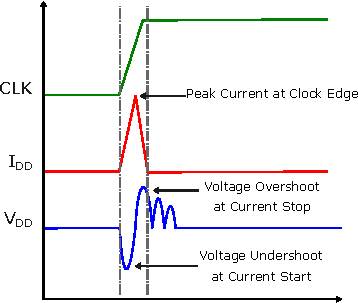
\includegraphics[scale=1.35, interpolate=false]
    {figures/villach-supply-analysis/chip-internal-oscillation}
    \caption[Chip-Internal Oscillation]{
        Chip-internal supply voltage oscillation at clock edges in a
        \ac{CMOS} circuit.
    }
    \label{fig:chip-internal-oscillation}
\end{figure}

In addition to the external power supply, the following factors contribute
to chip-internal voltage oscillations:

\begin{itemize}[topsep=8pt,itemsep=4pt,partopsep=4pt, parsep=4pt]
    \item
    The connection between external decoupling capacitors and on-chip
    switching nodes forms an effective RLC network, consisting of socket
    inductance, bond wire inductance and resistance, and chip-internal
    supply-to-ground capacitance \autocite{8919754}.

    \item
    Bond wire inductances limit the dynamic current delivery to the chip
    and convert fast load current transients into voltage drops and
    overshoots.

    \item
    Fast current transients generated at clock edges or during
    simultaneous switching events excite the RLC network, potentially
    leading to oscillatory behavior on internal supply rails.

    \item
    The slew rate of the load current determines the magnitude of the
    resulting voltage droop and subsequent voltage spike.

    \item
    Power-on and power-off transitions of internal power domains introduce
    additional current steps, which propagate through the chip-internal
    \ac{PDN} and package parasitics.

    \item
    Voltage droops become critical if the supply undershoot crosses
    digital noise margins for a duration sufficient to cause setup or
    hold time violations.
\end{itemize}

Low-impedance sockets, minimized bond wire inductance, and a well-designed
chip-internal \ac{PDN} help reduce internal voltage bounce. The speed and
stability of the \ac{DPS} control loop must be adapted to the overall
wiring length and parasitic elements of the test setup. Proper power
supply control loop design is therefore essential for reliable testing
and to minimize power-related anomalies.